\section{Benutzeroberfläche}%

Die GUI wird mit den Standard-""Oberflächenelementen der verwendeten Entwicklungsplattform (z.~B.\ Java, Eclipse Platform) gestaltet. Soweit anwendbar, folgt die Gestaltung den \emph{User Interface Guidelines} der verwendeten Plattform.

Die GUI soll für den mit der Plattform vertrauten Benutzer intuitiv benutzbar sein und häufig durchgeführte Arbeitsschritte beschleunigen.

\subsection{Prototyp der Editor-""Ansicht}%

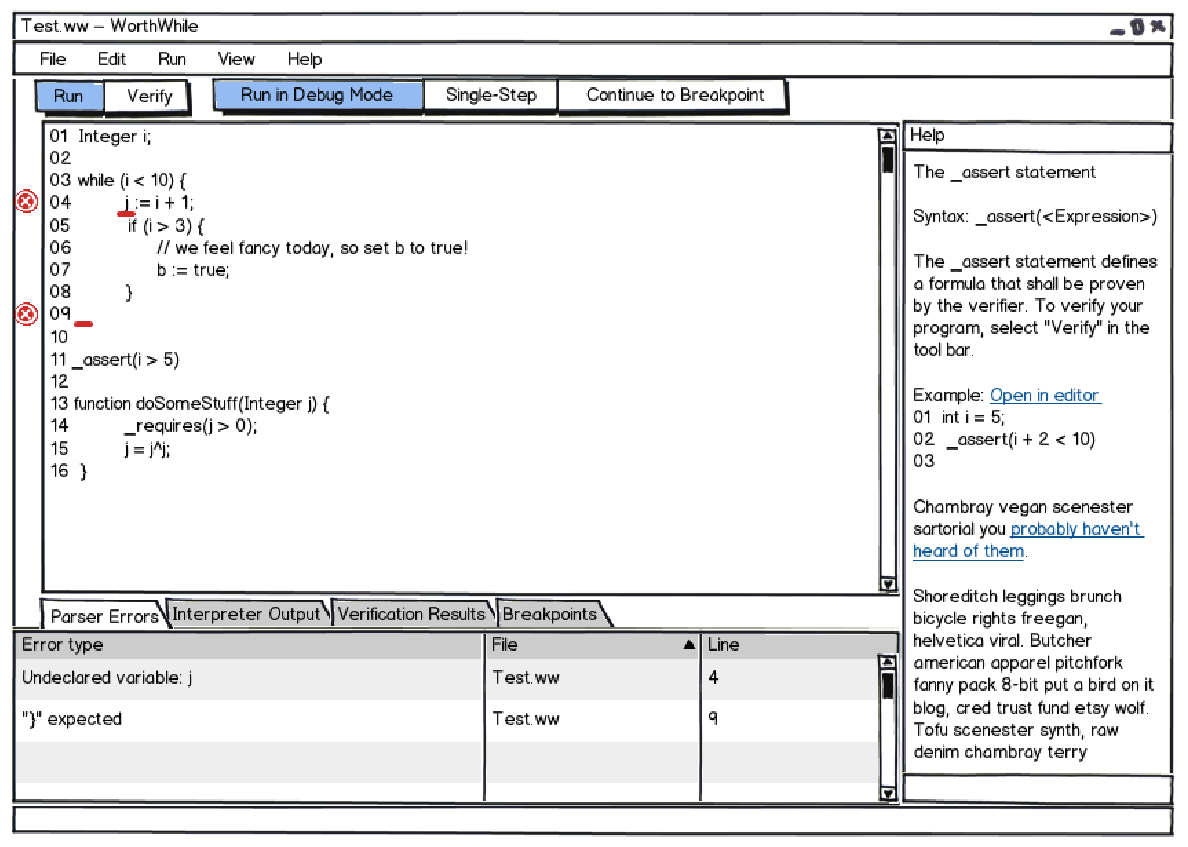
\includegraphics[width=\textwidth]{mockup/editor.pdf}

\subsection{Prototyp der Debugger-""Ansicht}%

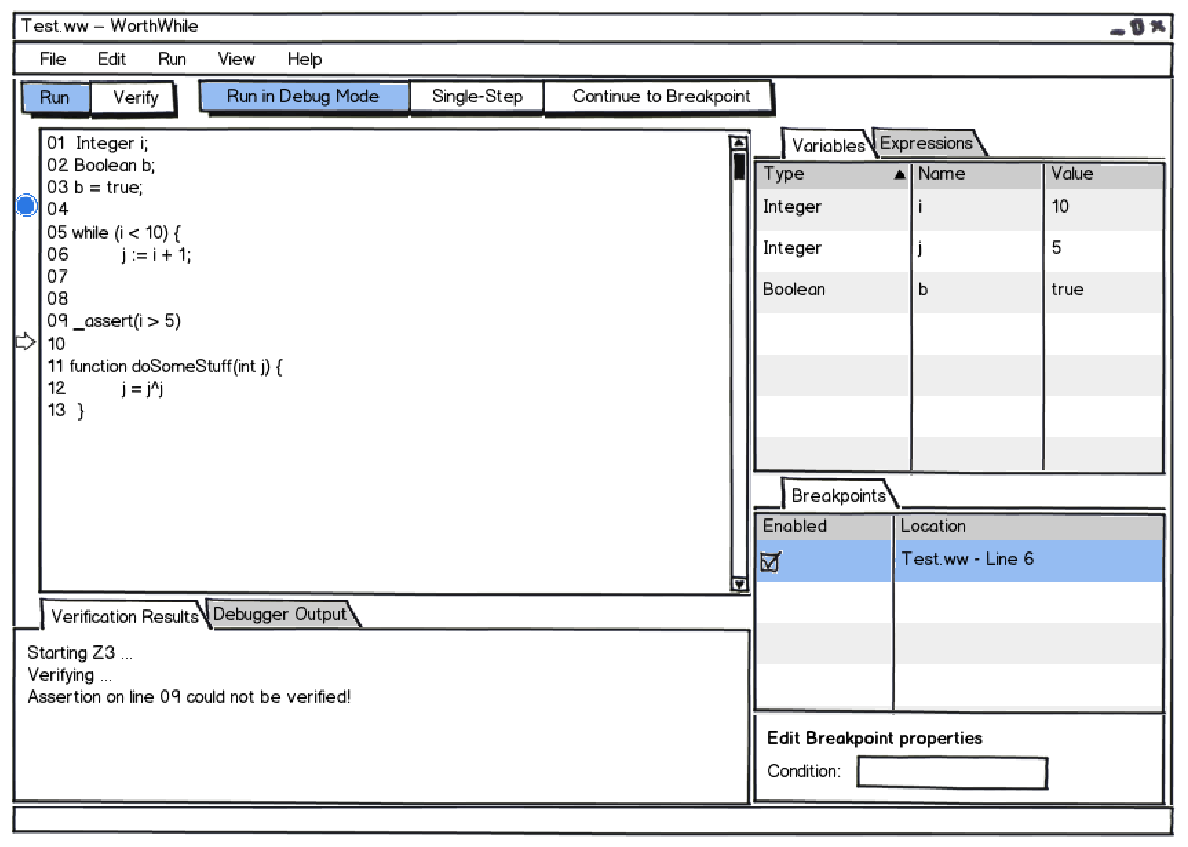
\includegraphics[width=\textwidth]{mockup/debug.pdf}
